\section{Einführung}
    \begin{itemize}
        \item[Bisher:] Wörter, d.h. gerichtete, zusammenhängende Grad1-Graphen\\
        oder: Funktion $\{1,\dots,n\}\rightarrow\Sigma$
        \item[jetzt:] Bäume
    \end{itemize}
    \subsection{Bäume}
        Was ist ein Baum?\\
        Graph mit folgenden Eigenschaften:
        \begin{itemize}
            \item azyklisch
            \item zusammenhängend (sonst ``Wald'')
            \item gerichtet
            \item gelabelte Knoten
            \item Rang (1 - Wörter, 2 - Binärbäume,\dots)\\
                je nach Definition:
            \begin{itemize}
                \item label-abhängig
                \item ohne Rang
            \end{itemize}
            \item endlich oder unendlich
        \end{itemize}
        Wir betrachten: endliche Binärbäume
    \subsection{Baumsprachen}
        Baumsprache $L\subseteq T^*_\Sigma$
\section{Knotenadressierung}
    \begin{itemize}
        \item bei Wörtern: $\{0,\dots,n\}\rightarrow\Sigma$
        \item bei Bäumen: $A\rightarrow\Sigma$
    \end{itemize}
    wobei $A\subseteq\{0,1\}^*,\ A$ abgeschlossen unter Präfixbildung und $w0\in A\Leftrightarrow w1\in A$
    \subsection{Beispiel}
        \begin{tikzpicture}[node distance=1.5cm]
            \node[state] (e) {$\epsilon$};
            \node[state] (0) [below left of=e] {0};
            \node[state] (00) [below left of=0] {00};
            \node[state] (01) [below right of=0] {01};
            \node[state] (010) [below left of=01] {010};
            \node[state] (011) [below right of=01] {011};
            \node[state] (1) [below right of=e] {1};

            \draw (e) -- (0);
            \draw (e) -- (1);
            \draw (0) -- (00);
            \draw (0) -- (01);
            \draw (01) -- (010);
            \draw (01) -- (011);
        \end{tikzpicture}
        \vspace*{-3cm}\\\hspace*{7cm}z.B. $t(01)=a$\vspace*{3cm}
\section{Konkatenation}
    im Gegensatz zu Wörtern nicht eindeutig:\vspace{-1cm}\\
    \begin{tikzpicture}[node distance=1.5cm]
        \node[state] (a) {};
        \node[state] (b) [below left of=a] {};
        \node[state] (c) [below right of=a] {};
        \node (cd) [above   right of=c]{$\cdot$};
        \draw (a) -- (b);
        \draw (a) -- (c);
    \end{tikzpicture}
    \begin{tikzpicture}[node distance=1.5cm]
        \node[state] (a) {};
        \node[state] (b) [below left of=a] {};
        \node[state] (c) [below right of=a] {};
        \node (cd) [above   right of=c]{$=$};
        \draw (a) -- (b);
        \draw (a) -- (c);
    \end{tikzpicture}
    \begin{tikzpicture}[node distance=1.5cm]
        \node[state] (a) {};
        \node[state] (b) [below left of=a] {};
        \node[state] (c) [below right of=a] {};
        \draw (a) -- (b);
        \draw (a) -- (c);
        \node[state] (a1) [below left of=b] {};
        \node[state] (b1) [below left of=a1] {};
        \node[state] (c1) [below right of=a1] {};
        \draw (a1) -- (b1);
        \draw (a1) -- (c1);

        \draw (b) -- (a1);
        \node (cd) [below right of=c]{$\leftarrow$ kein Binärbaum};
    \end{tikzpicture}
    \subsection{Kontexte}
        Idee: genau ein Blatt ist Loch ($\rightarrow$ ``Kontext'')\\
        \begin{tikzpicture}[node distance=1.5cm]
        \node[state] (a) {};
        \node[draw,rectangle,minimum size=0.5cm] (b) [below left of=a] {};
        \node[state] (c) [below right of=a] {};
        \node (cd) [above   right of=c]{$\cdot$};
        \draw (a) -- (b);
        \draw (a) -- (c);
    \end{tikzpicture}
    \begin{tikzpicture}[node distance=1.5cm]
        \node[state] (a) {};
        \node[state] (b) [below left of=a] {};
        \node[state] (c) [below right of=a] {};
        \node (cd) [above   right of=c]{$=$};
        \draw (a) -- (b);
        \draw (a) -- (c);
    \end{tikzpicture}
    \begin{tikzpicture}[node distance=1.5cm]
        \node[state] (a) {};
        \node[state] (c) [below right of=a] {};
        \draw (a) -- (b);
        \draw (a) -- (c);
        \node[state] (a1) [below left of=a] {};
        \node[state] (b1) [below left of=a1] {};
        \node[state] (c1) [below right of=a1] {};
        \draw (a1) -- (b1);
        \draw (a1) -- (c1);

        \draw (a) -- (a1);
    \end{tikzpicture}
\section{Baum-Automaten}
    \begin{itemize}
        \item analog zu DFA/NFA
        \item bei Wörtern:\\
            \begin{tikzpicture}[->]
                \node (q0) {$q_0$};
                \node (q1) [right of=q0] {$q_1$};
                \node (qi) [right of=q1] {\dots};
                \node (qn) [right of=qi] {$q_n$};
                \node (f) [right of=qn] {$\overset{?}{\in} F$};
                \draw (q0) edge[bend left] node[above]{$a$} (q1);
                \draw (q1) edge[bend left] node[above]{\dots} (qi);
                \draw (qi) edge[bend left] node[above]{\dots} (qn);
            \end{tikzpicture}
        \item bei Bäumen: Lauf ist ein Baum\\
            \begin{tikzpicture}
                \node (a) {a};
                \node (b) [below left of=a] {a};
                \node (c) [below right of=a] {b};
                \draw (a) -- (b);
                \draw (a) -- (c);
            \end{tikzpicture}
            Lauf:
            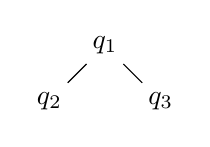
\begin{tikzpicture}
                \node (a) {$q_1$};
                \node (b) [below left of=a] {$q_2$};
                \node (c) [below right of=a] {$q_3$};
                \draw (a) -- (b);
                \draw (a) -- (c);
            \end{tikzpicture}
            \item es existieren bottom-up und top-down Automaten
            \item wir besprechen bottom-up
    \end{itemize}
    \subsection{Definition}
        nicht-deterministischer bottom-up Baumautomat:\\
        $\mathcal{A}=(Q,\Sigma,q_0,\delta,F)$
        \begin{itemize}
            \item $Q$ Zustände
            \item $\Sigma$ Alphabet
            \item $q_0$ Startzustand
            \item $\delta\subseteq Q\times Q\times \Sigma\times Q$ Übergangsrelation
            \begin{itemize}
                \item deterministisch: $\delta: Q\times Q\times \Sigma\rightarrow Q$
                \item top-down: $\delta\subseteq Q\times\Sigma\times Q\times Q$
            \end{itemize}
            \item $F\subseteq Q$ Endzustände
        \end{itemize}
        Sei $t\in T_\Sigma^*$. Ein Lauf $\rho$ auf $t$ erfüllt $$\left(\rho(w0),\rho(w1),t(w),\rho(w)\right)\in\delta,\ t: A\rightarrow\Sigma,\ \rho:A\rightarrow Q$$
        \subsubsection{Semantik}
            $L(\mathcal{A})=\{t\in T_\Sigma^*\mid\exists\rho\text{ Lauf auf }t:\rho(\epsilon)\in F\wedge w\text{ Blatt }\Rightarrow \rho(w)=q_0\}$
        \subsubsection{Determinisierung}
            Analog zu NFA$\rightarrow$DFA: Potenzmengenkonstruktion\\
            $\rightarrow$ Komplementabschluss
        \subsubsection{Definition}
            Baumsprache heißt regulär, wenn sie von Baumautomaten akzeptiert wird.
\section{Logik: $MSO$ und $FO$ auf Bäumen}
    \subsection{Syntax}
        \begin{itemize}
            \item $Q_ax$
            \item $x<y$
            \item $\neg\varphi$
            \item $\varphi\wedge\psi$
            \item $\exists x:\varphi$
            \item $\exists X:\varphi$
        \end{itemize}
        \subsubsection{Domäne}
            \begin{itemize}
                \item bei Wörtern: $\{0,\dots, n\}$
                \item bei Bäumen: $A\subseteq\{0,1\}^*$ (wie oben)
            \end{itemize}
            Prädikat $x<y, +1$ sinnvoll
        \subsubsection{Beispiel}
            \begin{tikzpicture}[node distance=1.5cm]
                \node[state] (a) {x};
                \node[state] (c) [below right of=a] {z};
                \draw (a) -- (b);
                \draw (a) -- (c);
                \node[state] (a1) [below left of=a] {};
                \node[state] (b1) [below left of=a1] {};
                \node[state] (c1) [below right of=a1] {y};
                \draw (a1) -- (b1);
                \draw (a1) -- (c1);

                \draw (a) -- (a1);
            \end{tikzpicture}
            $x<z,\ x<y$ aber nicht $z<x$ oder $y<z$
    \subsection{Satz}
        Für Baumsprachen gilt $MSO=$\textsc{Reg}. Beweis analog zu Wörtern.
\section{Baum-Grammatik}
    \subsection{Definition}
        $G=(V,\Sigma,P,S)$
        \begin{itemize}
            \item $V$ Variablen
            \item $\Sigma$ Alphabet
            \item $S\in V$ Startsymbol
            \item $P=\{A\rightarrow t\mid A\in V,\ t\in T_\Sigma^*\}$ wobei $V$ in $t$ nur an Blättern erlaubt ist.
        \end{itemize}
        $L(G)=\{t\in T_\Sigma^*\mid S\overset{P^*}{\rightarrow} t\}$
        \subsubsection{Beispiel}
            \begin{tikzpicture}[node distance=1.5cm]
                \node (A) {A};
                \node (ra) [right of=A] {$\rightarrow$};
                \node (B) [below right of=ra] {B};
                \node (a) [above right of=B] {a};
                \node (b) [below right of=a] {b};
                \draw (a) --(b);
                \draw (a) -- (B);
            \end{tikzpicture} dann:\\
            \begin{tikzpicture}[node distance=1.5cm]
                \node (a1) {a};
                \node (b1) [below left of=a1] {b};
                \node (A) [below right of=a1] {A};
                \node (ra) [right of=A] {$\rightarrow$};
                \node (b2) [right of=ra] {b};
                \node (a2) [above right of=b2] {a};
                \node (a) [below right of=a2] {a};
                \node (B) [below left of=a] {B};
                \node (b) [below right of=a] {b};
                \draw (a) --(b);
                \draw (a) -- (B);
                \draw (a1) -- (b1);
                \draw (a1) -- (A);
                \draw (a2) -- (b2);
                \draw (a2) -- (a);
            \end{tikzpicture}
    \subsection{Satz}
        Baumsprache $L$ regulär $\Leftrightarrow\exists$ Grammatik $G$ mit $L(G)=L$
    \subsection{Definition: yield}
        Sei $t\in T_\Sigma^*$, dann ist  $yield:\ T_\Sigma^*\rightarrow\Sigma^*$ die Blattsprache.
        \subsubsection{Beispiel}
            $t:$\begin{tikzpicture}[node distance=1.5cm]
                \node (b2) {b};
                \node (a2) [above right of=b2] {a};
                \node (a) [below right of=a2] {a};
                \node (B) [below left of=a] {a};
                \node (b) [below right of=a] {b};
                \draw (a) --(b);
                \draw (a) -- (B);
                \draw (a2) -- (b2);
                \draw (a2) -- (a);
            \end{tikzpicture}
            $yield(t)=bab$
    \subsection{Satz}
        $L$ kontextfrei $\Leftrightarrow\exists K\subseteq T_\Sigma^*$ reg mit $yield(K)=L$
        \subsubsection{Anmerkung}
            \begin{itemize}
                \item Bäume, reguläre Sprachen: $NC^1$
                \item CFL, $yield$s: $SAC^1$
            \end{itemize}
        \subsection{Beweis}
            \begin{itemize}
                \item[$\Leftarrow$:] Sei $G'$ Grammatik mit $L(G')=K$. Konstruiere kontextfreie Grammatik $G$ mit $L(G)=L=yield(K)$. $G'=(V,\Sigma,S,P')$, dann $G=(V,\Sigma,S,P)$ mit $P=\{A\rightarrow yield(t)\mid A\rightarrow t\in P'\}$.\\Es ist $yield(t)=yield(t_1)yield(t_2)$, wenn $t=$\vspace*{-.5cm}\\\hspace*{7cm}\begin{tikzpicture}
                    \node (a) {a};
                    \node (t1) [below left of=a] {$t_1$};
                    \node (t2) [below right of=a] {$t_2$};
                    \draw (a) -- (t1);
                    \draw (a) -- (t2);
                \end{tikzpicture}\\
                Somit gilt für Satzform:\\
                $t\overset{P'}{\rightarrow}t'\Leftrightarrow yield(t)\overset{P}{\rightarrow} yield(t')$\\
                induktiv gilt: $t\in L(G')\Leftrightarrow yield(t)\in L(G)$
                \item[$\Rightarrow$] Sei $L$ CFL.\\
                $\Rightarrow\exists G=(V,\Sigma,P,S)$ in CNF mit $L=L(G)$\\
                Konstruiere $G'$ mit $yield(L(G'))=L$\\
                Für jede Regel in $G$\begin{itemize}
                    \item der Form $A\rightarrow a$ füge in $G'$ ein $A\rightarrow$\begin{tikzpicture}
                        \node[state] (a) {a};
                    \end{tikzpicture}
                    \item der Form $A\rightarrow BC$ füge in $G'$ ein $A\rightarrow$\begin{tikzpicture}[node distance=1.5cm]
                        \node[state] (a) {a};
                        \node[state,below left of=a] (B) {B};
                        \node[state,below right of=a] (C) {C};
                        \draw (a) -- (B);
                        \draw (a) -- (C);
                    \end{tikzpicture}
                \end{itemize}
                induktiv folgt $yield(L(G'))=L$\qed
            \end{itemize}
